%! Licence = CC BY-NC-SA 4.0

%! Author = gianfluetsch
%! Date = 30. Dez 2021
%! Project = cydef_summary

\section{Yara}
YARA (Yet Another Recursive/ Ridiculous Acronym) ist ein Tool, das Malware-Forschern bei der Identifizierung und Klassifizierung von Malware-Mustern helfen soll (aber nicht darauf beschränkt ist). Mit YARA können Sie Beschreibungen von Malware-Familien (oder was auch immer Sie beschreiben möchten) auf der Grundlage von textuellen oder binären Mustern erstellen. Jede Beschreibung, auch als Regel bezeichnet, besteht aus einer Reihe von Zeichenketten und einem booleschen Ausdruck, die ihre Logik bestimmen.

\subsection{Allgemein}
\begin{itemize}
    \item Identifying malware: hash code
    \begin{itemize}
        \item Problem: very restrictive
        \item Changing one bit $\rightarrow$ different hash
    \end{itemize}
    \item Alternative:
    \begin{itemize}
        \item Identify “marker” patterns
        \item Standard: YARA rules
    \end{itemize}    
\end{itemize}
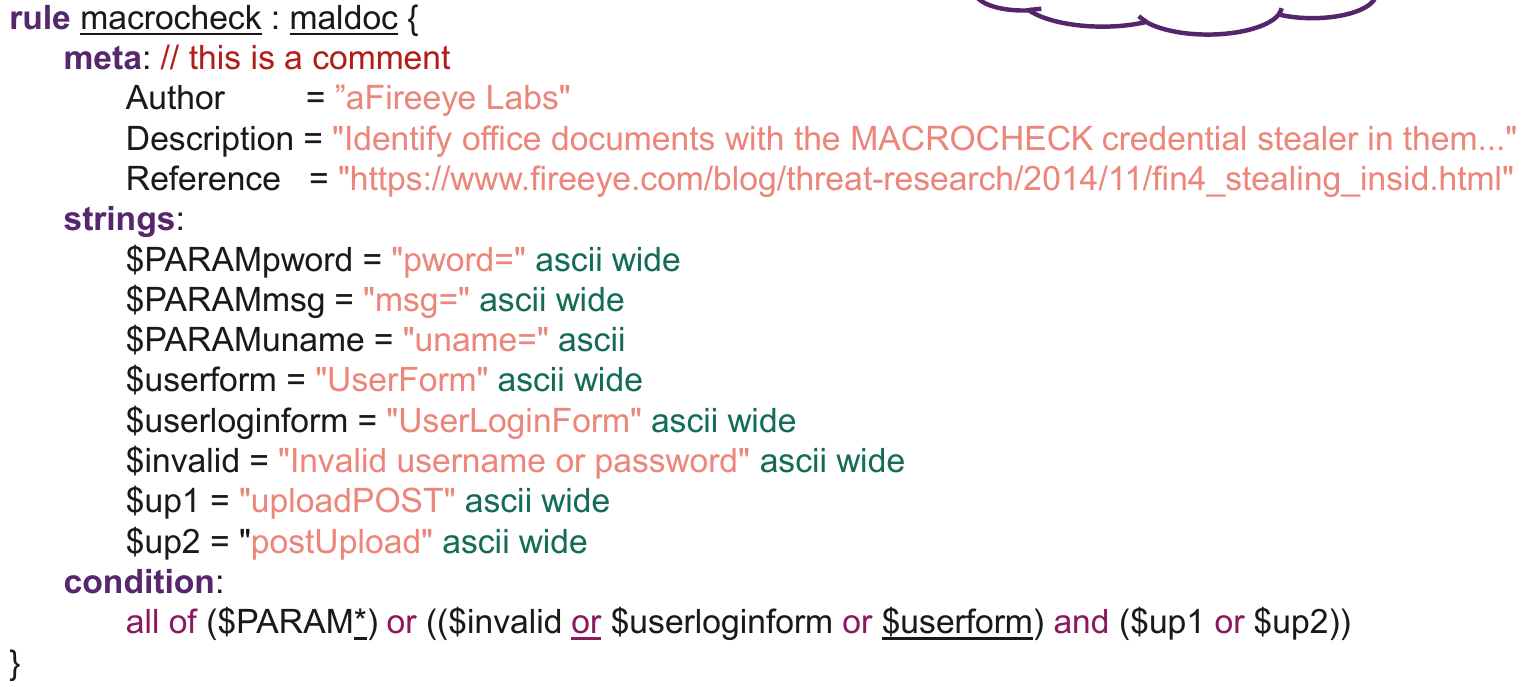
\includegraphics[width=\linewidth]{./img/13-yara/yara_rule.png}
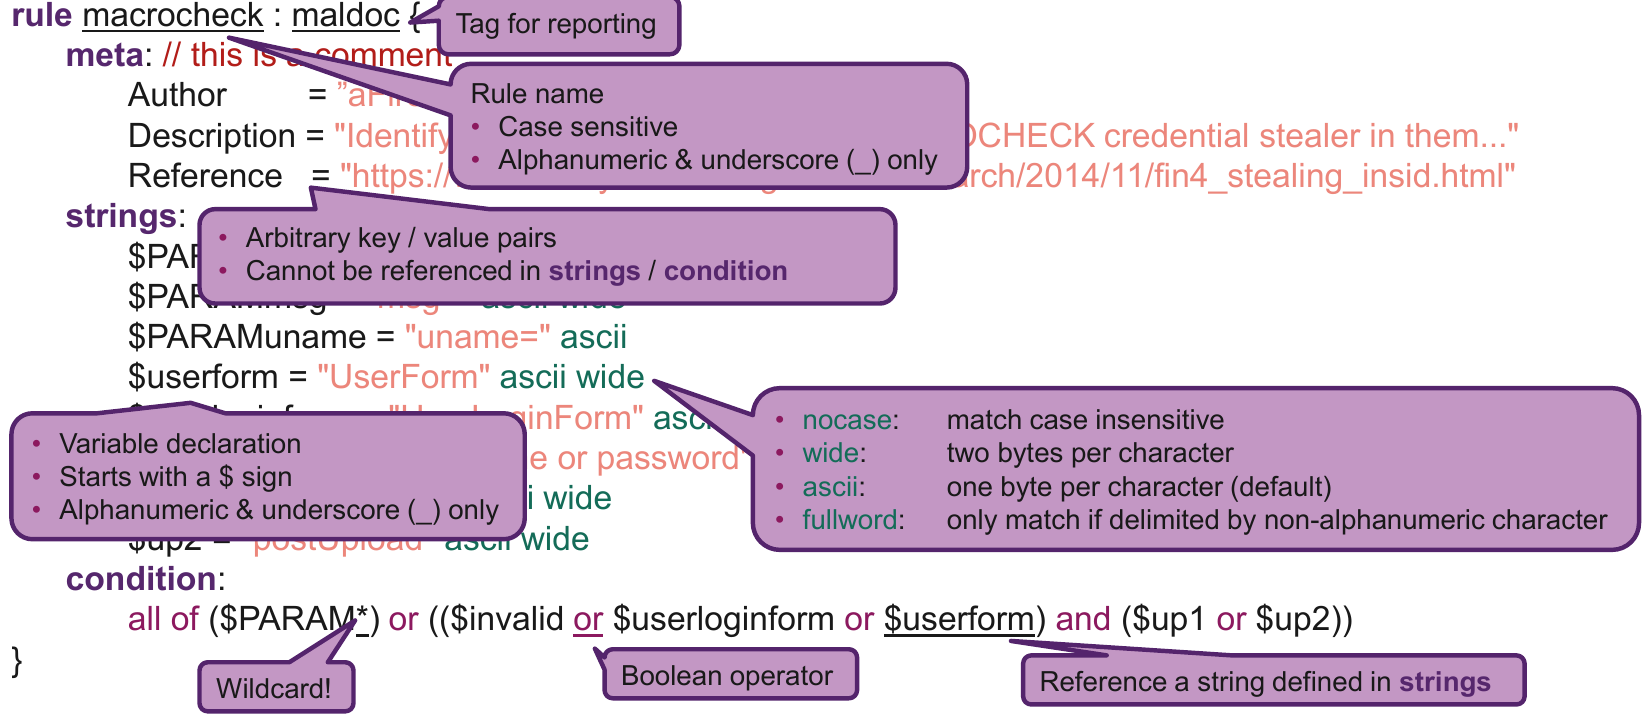
\includegraphics[width=\linewidth]{./img/13-yara/yara_rule_explained.png}
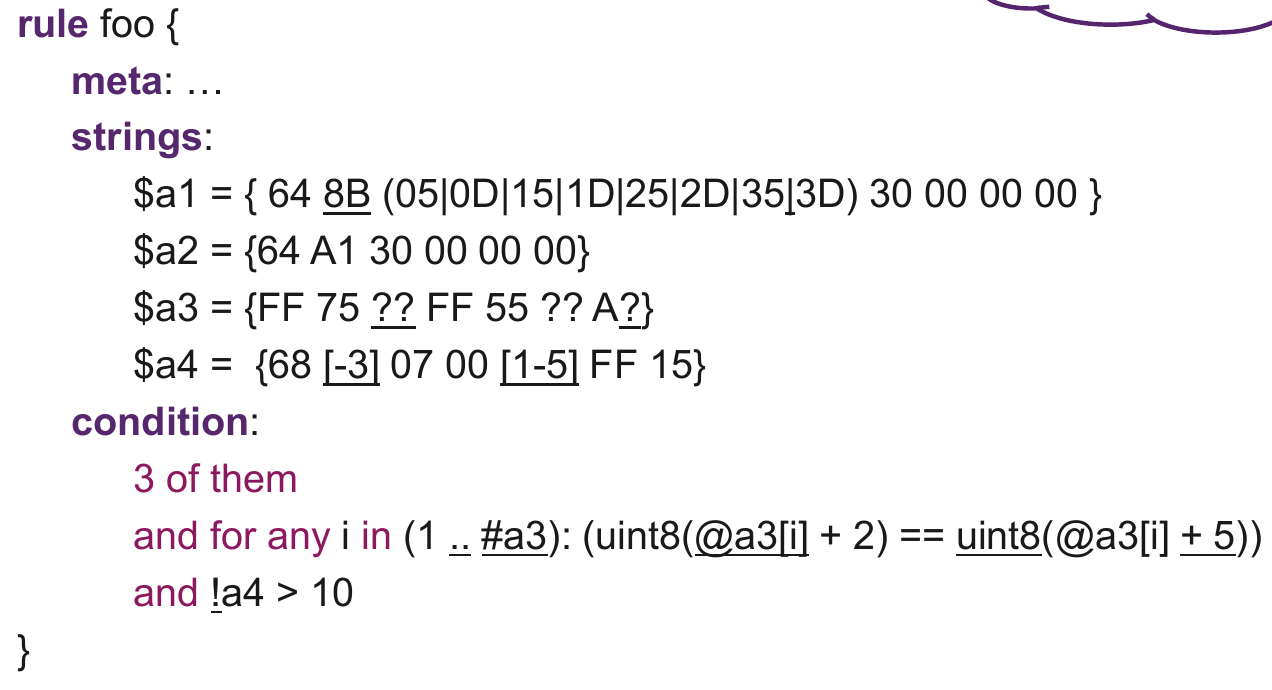
\includegraphics[width=\linewidth]{./img/13-yara/yara_rule2.png}
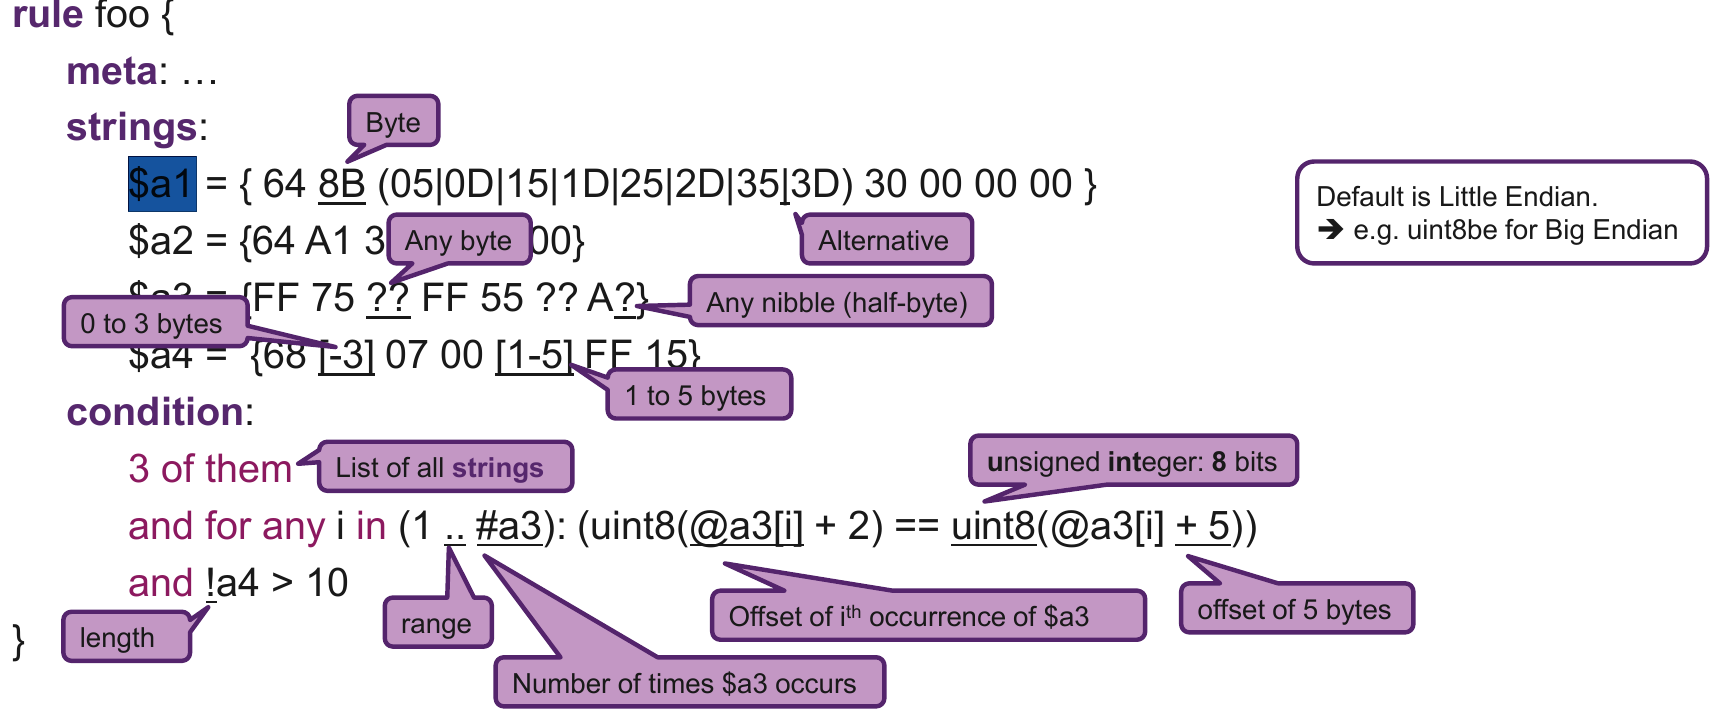
\includegraphics[width=\linewidth]{./img/13-yara/yara_rule_explained2.png}
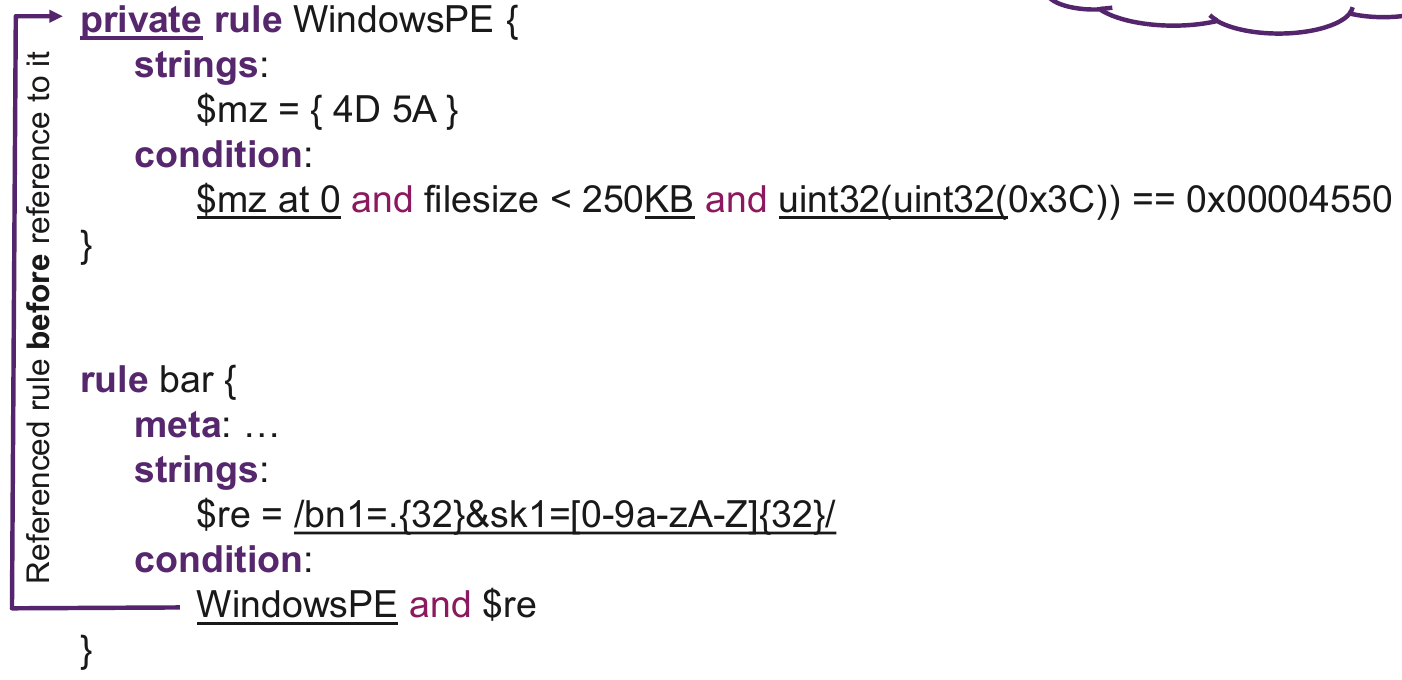
\includegraphics[width=\linewidth]{./img/13-yara/yara_rule3.png}
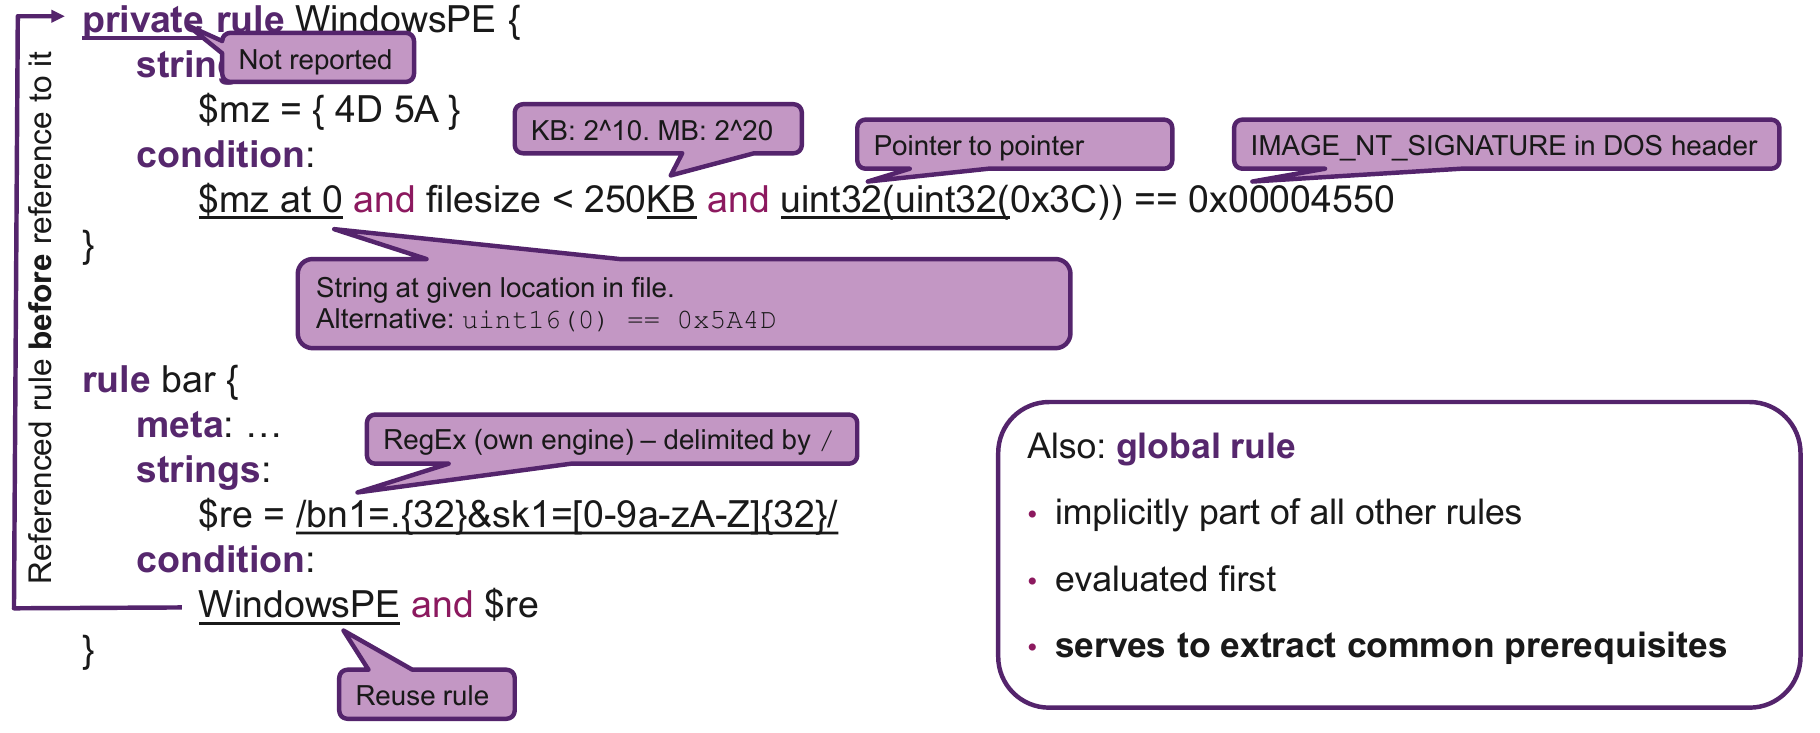
\includegraphics[width=\linewidth]{./img/13-yara/yara_rule_explained3.png}
Wenn mit yara gesucht wird, \textbf{matcht eine "private rule" NIE!}
\begin{itemize}
    \item sondern immer nur die globale rule (in diesem Bsp ''bar'')
    \item in der globale rule ''bar'' kann als condition aber die private rule (WindowsPE) hinterlegt werden!\\
\end{itemize}
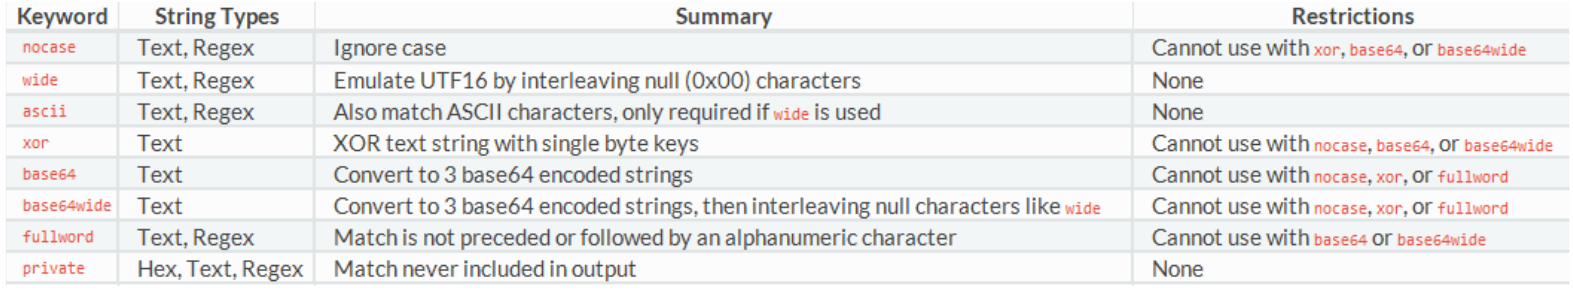
\includegraphics[width=\linewidth]{./img/13-yara/yara_string.png}

\subsection{Packer}
\begin{itemize}
    \item Most malware today is packed in some way to help get around AV signature detection
    \item There are over 8000 known packers out there, each with their own signatures.
    \item They can range from simple compression to full on encryption / debugger detection and generally make the life of the Malware Reverser a pain.
    \item Packers are not fool proof – the exe HAS to be decrypted / decompressed at SOME point in order to run on the OS.
\end{itemize}
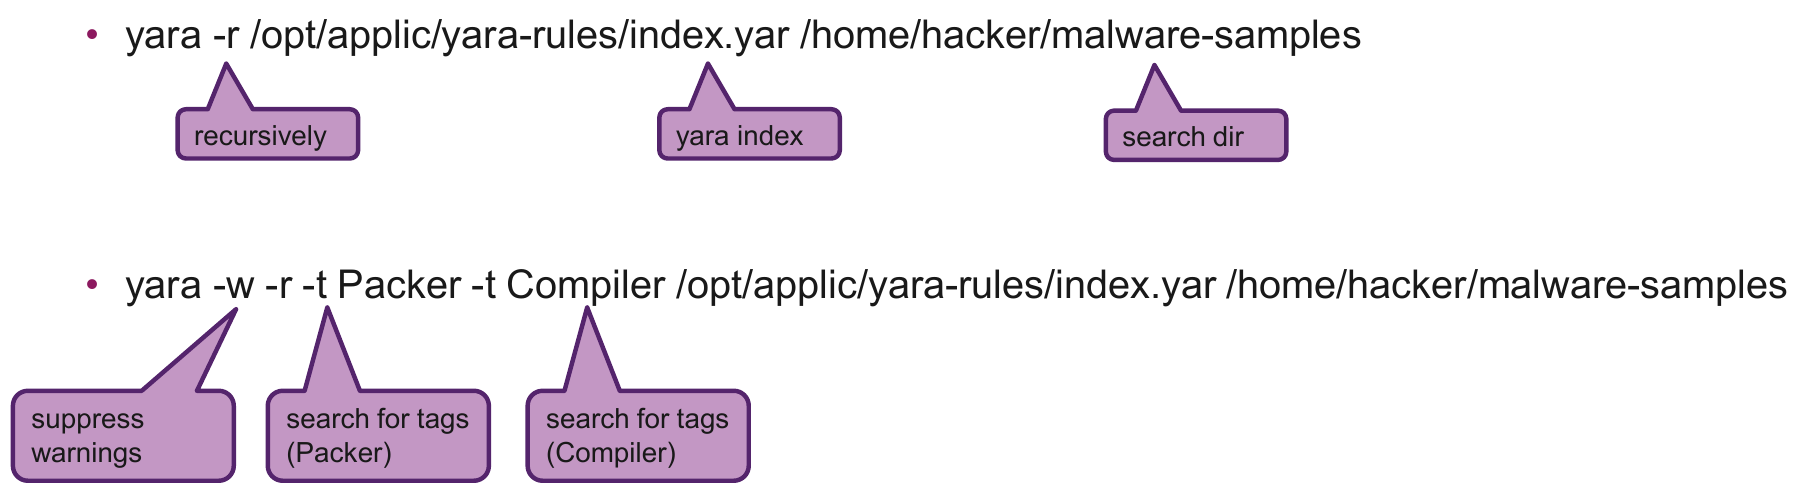
\includegraphics[width=\linewidth]{./img/13-yara/yara_cli.png}

\subparagraph{Yara \& Volatility}
\subsection{Yara and yarGen}

\subsubsection{Awesome Yara}
\textit{Awesome Yara} is a list of yara rules, tools and resourced inspired by awesome-python and awesome-php.

\subsubsection{yarGen}
\textit{yarGen} is a generator for YARA rules

The main principle is the creation of yara rules from strings found in malware files while removing all strings that also appear in goodware files. Therefore \textit{yarGen} includes a big goodware strings and opcode database as ZIP archives that have to be extracted before the first use.

\subsection{tcpdump and Yara}

\subsubsection{tcpflow}
\textit{tcpflow} is a free, open source, powerful command line based tool for analyzing network traffic on Unix-like systems. It captures data received or transferred over TCP connections, and stores it in a file for later analysis, in a useful format that allows for protocol analysis and debugging.

The following command will extract files from the pcap dump to the ./output folder
\begin{lstlisting}[language=bash]
    tcpflow -r pcap-file.pcap -o ./output
\end{lstlisting}

After the extraction, you can see the \textit{md5sum} (hash) of the malware.

\subsubsection{NetworkMiner}
\textit{NetworkMiner} is an open source Network Forensic Analysis Tool (NFAT). \textit{NetworkMiner} can be used as a passive network sniffer/packet capturing tool in order to detect operating systems, sessions, hostnames, open ports etc. without putting any traffic on the network. \textit{NetworkMiner} can also parse PCAP files for off-line analysis and to regenerate/reassemble transmitted files and certificates from PCAP files.\\

\textit{NetworkMiner} is like tcpflow a tool to extract files from the pcap dump.
In contrast to tcpflow, \textit{NetworkMiner} is a graphical tool for this.

After the extraction, you can see the \textit{md5sum} (hash) of the malware.

\subsubsection{chaosreader}
Another method of extracting the file from the pcap is \textit{chaosreader}.\\

A freeware tool to trace TCP/UDP/... sessions and fetch application data from snoop or tcpdump logs. This is a type of \glqq any-snarf\grqq program, as it will fetch telnet sessions, FTP files, HTTP transfers (HTML, GIF, JPEG, ...), SMTP emails, ... from the captured data inside network traffic logs. A html index file is created that links to all the session details, including realtime replay programs for telnet, rlogin, IRC, X11 and VNC sessions; and reports such as image reports and HTTP GET/POST content reports.

\begin{lstlisting}[language=bash]
    /usr/bin/chaosreader -v pcap-file.pcap
\end{lstlisting}

\subsubsection{binwalk}
\textit{Binwalk} is a fast, easy to use tool for analyzing, reverse engineering, and extracting firmware images.

\begin{lstlisting}[language=bash]
    binwalk -e pcap-file.pcap
\end{lstlisting}

